\chapter{Evaluation}
%importance of evaluation
Evaluation is important to assess the ability and design of visuals in achieving their purpose. We conducted a user study to evaluate the system and its effectiveness at facilitating collaborative feature selection. In this chapter, we first outline the purpose and focuses of the evaluation and then explain its procedure. Later in this chapter, we describe the series of tasks that make up the study, explain how the tasks evaluate the system and explain the results of the tasks.

\section{ Objectives of the Evaluation Study }
The three main foci of the evaluation study aimed to understand the user interface's effectiveness at facilitating collaborative feature selection and the interpretability of the visualizations. Qualitative and quantitative evaluation methods are utilized to answer specific research questions.

\subsection{Research Questions}
Specific research questions extend from the main foci of the evaluation study. The research questions for the study are organized into three categories - effectiveness of the system, interpretability of the visualizations, and the exploration of feature space. The research questions are listed below.

Effectiveness measures the ability of the user interface to help the user accomplish their task.
\begin{itemize}
\item{Is the design of the application intuitive to the user?}
\item{Does the user build a classifier with high performance?}
\item{Does the built classifier reflect causal aspects accurately?}
\item{Does the built classifier reflect feature importance accurately?}
\end{itemize}

Interpretability measures the ability of the visuals to correctly and efficiently communicate information.
\begin{itemize}
\item{Are the visuals produced by the application easy to read?}
\item{Are the visuals correctly analyzed by the user?}
\item{Can the user explain/interpret the feature set used to build the classifier? }
\item{Can the user explain/interpret why a certain feature set may create a higher performing classifier than another feature set?}
\item{Does each piece contribute to the overall interpretability? I.e. if the causal graph is removed, is it more difficult to explain the classifier’s performance?}
\end{itemize}

Exploration of feature space measures the ability of the application to help the user make feature selections and identify a subspace of predictive feature sets.
\begin{itemize}
\item{Does the design of the application aid in feature exploration?}
\item{How quickly can a user select the most relevant features?}
\item{How quickly can a user filter out the most irrelevant features?}
\item{How quickly can the user choose between features that directly influence the label versus indirectly influence the label?}
\end{itemize}

\section { Methodology }
\subsection { Version B }
For the evaluation study, we create a separate application that does not incorporate prior knowledge about feature importance or causal relationships. The original application will be referred to as version A and the participants using version A are in group A, while the limited application will be referred to as version B and those participants are in group B.

The only two steps in version B are feature selection and performance analysis as shown in figures \ref{fig:LabelFSInterface} and \ref{fig:PerformanceAnalysisPage}. Group B's behavior and responses are compared against group A's to determine the effects that integrating prior knowledge has on feature selections, the number of trials performed during feature selection, the total time for the feature selection process, and other behaviors.

\subsection{ Participants }
Participants are recruited from the undergraduate and graduate students at Case Western Reserve University. First, they are provided with a high-level overview of the study and consent to participating in the study and having unidentifiable data collected. Participants then answer a questionnaire about their major and knowledge of machine learning and classification, which is used to divided them equally into group A and group B. When assigning participants to a group, we match two participants with similar characteristics and divide them between the two groups. The characteristics we use to match participants are major, age, and experience in machine learning. Participants in group A and B are further specified based on whether they majored in computer science (CS) or not. The number of participants in and information about group A and B are presented in table \ref{ParticipantInfo}.

\begin{table}[]
\centering
\begin{tabular}{lcc}
\hline
Participants &  \multicolumn{1}{l}{Version A} &  \multicolumn{1}{l}{Version B} \\ \hline
CS           & 10        & 5        \\
Other       & 5         & 5         \\ \hline
\textbf{Total}        & \textbf{15}        & \textbf{10}        \\ \hline
\end{tabular}
\caption{Participants are grouped by which system they are evaluating and whether they major in CS or not. The number of participants in each group is reported. }
\label{ParticipantInfo}
\end{table}

\subsection {Design of the Evaluation}
The system is designed for users with basic knowledge and understanding of machine learning and classification. In the introductory material (figures \ref{fig:IntroMaterials1}, \ref{fig:IntroMaterials2}), participants are given brief explanations about classification and feature selection, an example of a use case for the system, and necessary terminologies - such as accuracy, target label, etc. They are trained through a series of short introductory videos that explain the feature selection workflow, the system functionalities, and the interface visualizations. The tutorial features a weather classification problem that is classifying tomorrow's weather conditions as either sunny, rainy, or foggy based on today's weather metrics. After processing the introductory materials, participants interact with the system that shows the demonstration dataset. After they are familiarized with the system, they proceed to the user study.

\begin{figure}
    \centering
    \begin{minipage}{0.5\textwidth}
        \centering
        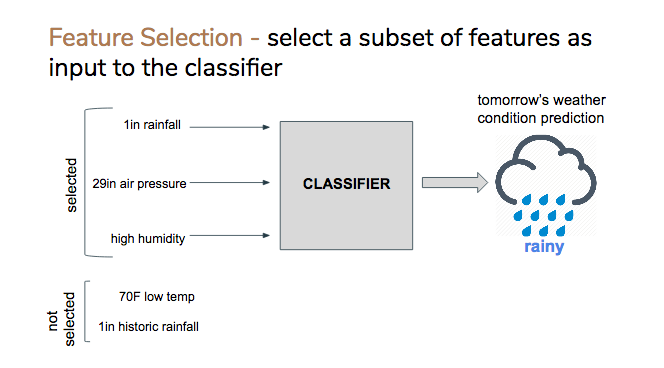
\includegraphics[width=.85\textwidth]{intromaterial1}
    \end{minipage}\hfill
    \begin{minipage}{0.5\textwidth}
        \centering
        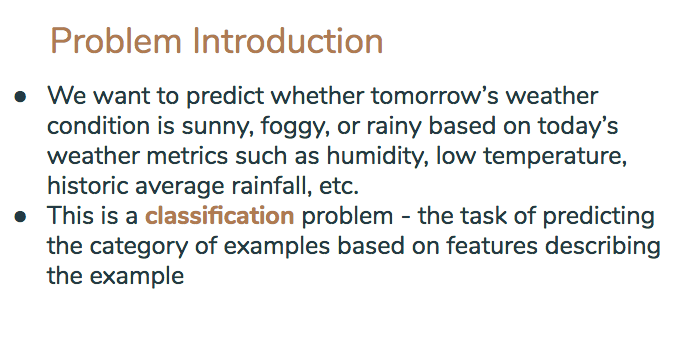
\includegraphics[width=1\textwidth]{intromaterial2}
    \end{minipage}
    \caption{\textbf{Introductory Material}. (Left) The slide introducing the demonstration classification example - predicting tomorrow's weather condition using today's weather condition. (Left) The slide explaining feature selection using the demonstration example. }
    \label{fig:IntroMaterials1}
\end{figure}

\begin{figure}
    \centering
    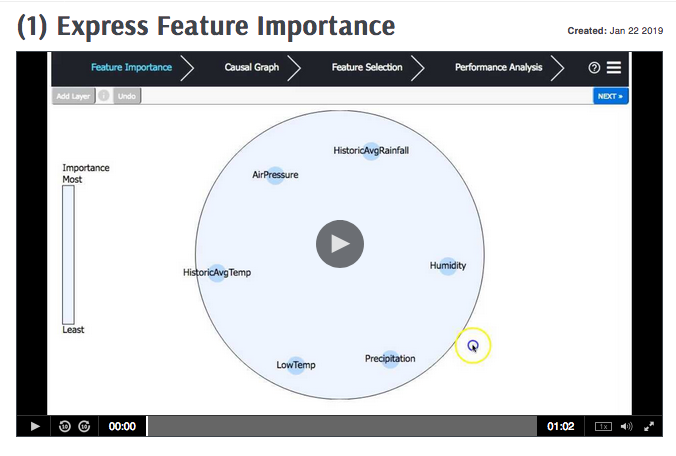
\includegraphics[width=.85\textwidth]{intromaterial3}
    \caption{\textbf{Demonstration Video}. Participants watched a series of videos that explained the user interface and system functionalities. The first video the participants watched was on expressing feature importance. }
    \label{fig:IntroMaterials2}
\end{figure}

\subsection { Gathering User Interaction Data }
During the evaluation process, a tracking mechanism traces the participant's actions such as interactions with the graph, edits to the graph, moving features to a different circle, etc. Using the tracking mechanism, we can measure the time spent on each task, record the interactions performed to accomplish each task, and the correctness of their answer. The events are tracked and logged by keen \cite{keen}, an application for tracking and analyzing user interactions. Events are analyzed to extract quantitative results about the effectiveness and usability of the system.

Some tasks require the participants to interact with the interface, such as ``You think that today's humidity is important for predicting tomorrow's weather. Express this knowledge using the system". In addition, some tasks require written responses to understand if the participants correctly interpret the visualizations - such as ``What are the Markov blanket features of the target variable".

\section { Background Information }
The participants were presented with a specific scenario. The participants were told that they are developing a classifier for predicting student's letter grades (A, B, C, or F) based on information about the student such as whether they work a part-time job or participate in extracurricular. They were instructed to first read the descriptions of each feature which are presented in the sidebar of the application, as shown in figure \ref{fig:featuredescriptions}. Feature and the target variable descriptions presented to the participants are shown in table \ref{featuredescription}.

\begin{figure}
    \centering
    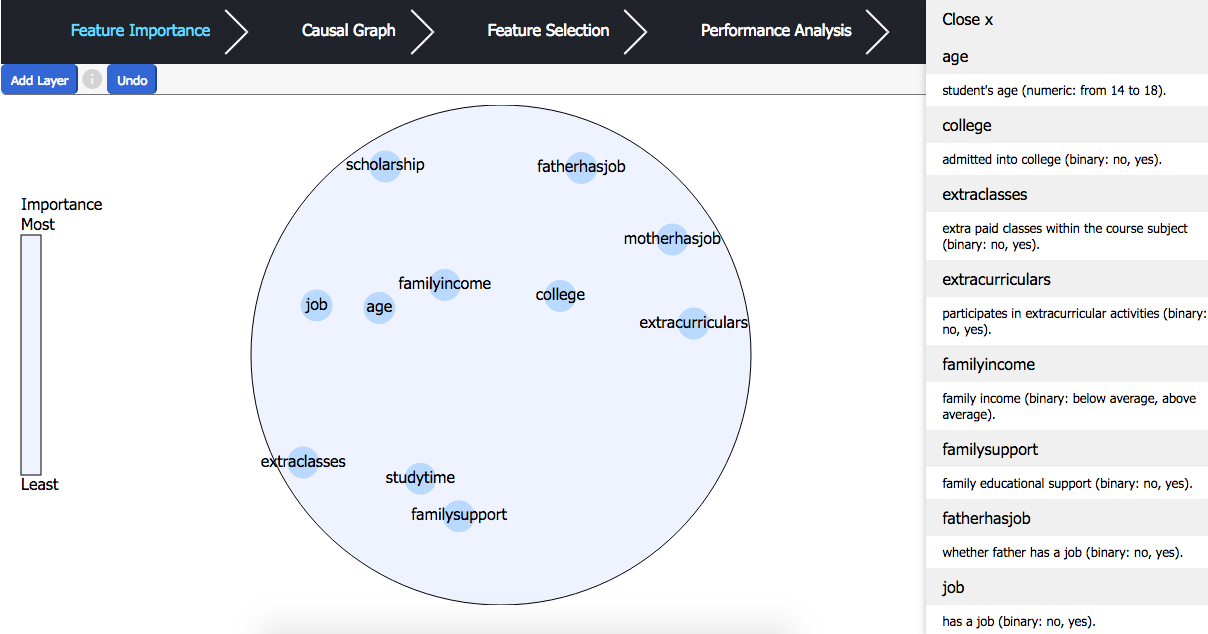
\includegraphics[width=.8\textwidth]{featuredescriptions}
    \caption{\textbf{ Feature Descriptions }. Participants were instructed to read feature descriptions presented on the sidebar of the interface. }
    \label{fig:featuredescriptions}
\end{figure}

\begin{table}[]
\centering
\begin{tabular}{lll}
\hline
Variables & Description & Values \\ \hline
motherhasjob & whether mother has a job & no, yes \\
extracurriculars& participates in extracurriculars & no, yes \\
job & has a job & no, yes \\
studytime & weekly study time & $>$2hr, 2-5hr, 5-10hr, $<$10hr \\
age & student's age & 14 to 18 \\
fatherhasjob & whether father has a job & no, yes \\
familyincome & family income & below avg, above avg \\
extraclasses & take extra classes & no, yes \\
familysupport & family educational support & no, yes \\
college & admitted into college & no, yes \\
scholarship & has scholarship for college & no, yes \\
grade & student letter grade & A B C F \\ \hline
\end{tabular}
\caption{Description of the features presented to the participants before they started the tasks.}
\label{featuredescription}
\end{table}

\subsection { Data Generation }
The dataset used for the evaluation study was generated from a Bayesian network created in pgmpy \cite{pgmpy}, a python library for working with probabilistic graphical models. First, the edges to and from variables representing features are defined. Then, the conditional probability distribution for each variable is defined. The actual Bayesian network that generated the data is shown in figure \ref{fig:actualBN}. 

After the Bayesian network is created, we generate samples from joint distribution of the Bayesian network. 500 examples are sampled from the Bayesian network to create the evaluation data set. 

\begin{figure}
    \centering
    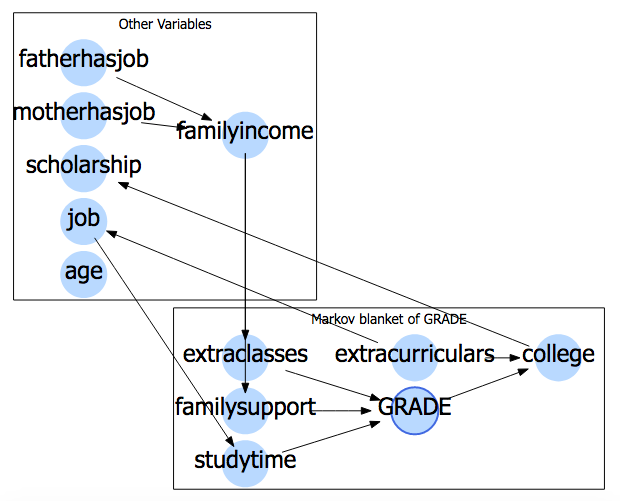
\includegraphics[width=.8\textwidth]{actualBN}
    \caption{\textbf{ Actual Bayesian Network of Evaluation Data set.}}
    \label{fig:actualBN}
\end{figure}

\subsection{ Evaluation Study Classification }
The interactive feature selection system is designed to be model agnostic. In theory, the user will be able to specify the classification algorithm and its parameters. For the evaluation study, we use the k-nearest neighbors algorithm (kNN) for classification and set the number of nearest neighbors $k$ to use as 3. kNN assigns an example to the target label that is most common among its $k$ nearest neighbors.

Moreover, we perform stratified 5 fold cross validation. The original dataset is randomly partitioned into 5 equal sized subsets where the fractions of target labels equal that of the original data set. Of the 5 subset, a single set is retained for testing the resulting classifier; the remaining 4 sets are used as training data to create the classifier. The cross-validation process is repeated 5 times. Each of the subsets is used once as testing data. Lastly, the 5 results such as test accuracy is averaged to produce the overall test accuracy.

\section { Evaluation Study }
We describe the background information presented to the participants and the instructions for each of the evaluation tasks.

The participants were told they will complete a series of tasks that will guide them to select features that will predict student grades. The tasks evaluate the feature selection process and the results will help answer the research questions. The tasks will be described later in this section. The tasks were presented one after the other and were to be completed consecutively. If the participant was unable to answer the question using the system or did not want to perform a task, they could proceed onto the next task without completing the task.

\subsection { Task 1: Express Feature Importance }
After the participants finished reading the feature descriptions, they proceeded to the first task. Task 1 evaluates the express feature importance step. 

Participants were informed that whether a student takes extra classes may be important for predicting their grade and that whether a student is admitted to college may be important but not as important as whether they take extra classes. 

Participants were instructed to express the importance of these features as well as their own ideas about which features are important for predicting student grades. The placement and grouping of features were logged and compared against the information provided in the task. This task was only completed by group A. 

Task 1 assesses the effectiveness of the interface and its interactions at helping the user express feature importance. Task 1 also evaluates the intuitiveness of the visualization and interactions. 

\begin{figure}
    \centering
    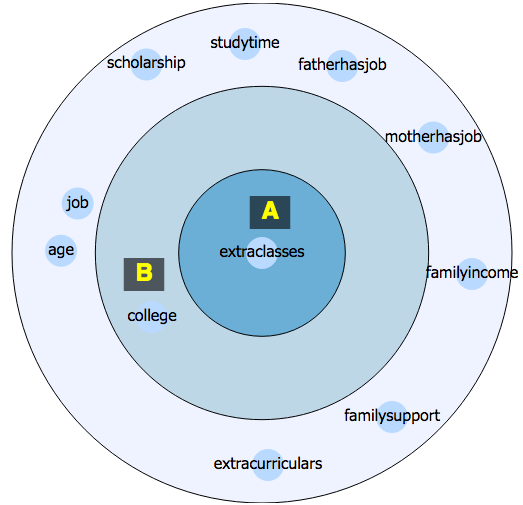
\includegraphics[width=.65\textwidth]{task1}
    \caption{\textbf{ Express Feature Importance Task }. The correct execution of the task places (A) extraclasses, the most important feature, in the innermost circle and (B) college in the adjacent circle. }
    \label{fig:Task1}
\end{figure}

\subsection { Task 2: Edit and Build Causal Graph }
The participants were then instructed to proceed to the next step which was expressing causal relationships. The GES algorithm outputted a possible causal network and the system presented the network to the participant. 

The participants were asked to utilize the functionalities of the interface to edit the causal graph. They were asked to express that participating in extracurricular is a cause of having a part-time job and having family support is a cause of participating in extracurricular. Moreover, if there are relationships that did not make sense or seems backward, the participant could remove or reverse the edge. The participant could also add edges to represent relationships. A possible causal network after the participants completed the task is presented in figure \ref{fig:Task2}. This task was only completed by group A. 

Task 2 is design to test the effectiveness of the interface and interactions at helping the user express causal relationships and build a causal network. 

\begin{figure}
    \centering
    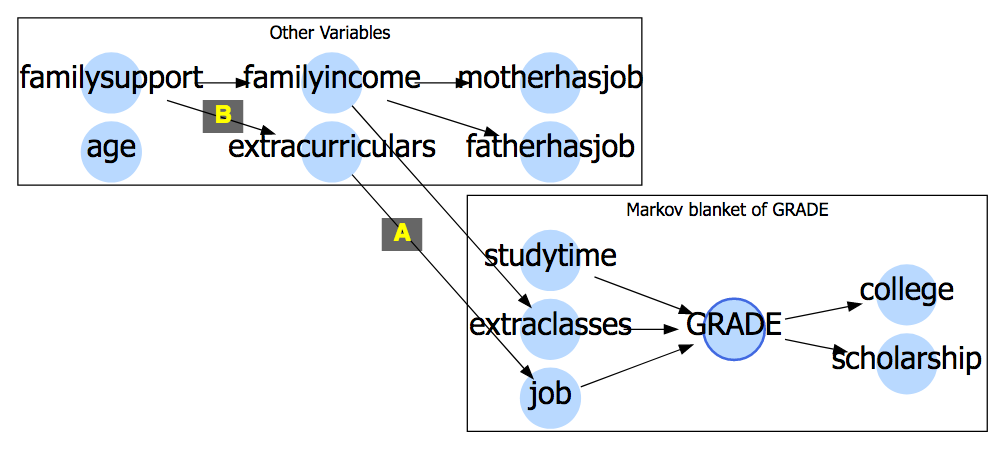
\includegraphics[width=.85\textwidth]{task2-2}
    \caption{\textbf{ Build Causal Graph Task }. A possible causal network of the dataset after the participant edit the graph to show (A) participating in extracurriculars as a cause of having a job and (B) having family support as a cause of participating in extracurriculars. The indirect causes of student grades are family income, family support, and extracurriculars. There are no indirect effects of student grades.}
    \label{fig:Task2}
\end{figure}

\subsection { Task 3: Interpret Causal Graph }
Task 3 was to be completed at the build causal network step. Participants were asked to identify indirect causes and effects of grade by reading and interacting with the graph. In figure \ref{fig:Task2}, the indirect causes of student grades are family income, family support, and extracurriculars and there are no indirect effects of student grades. This task is only completed by group A. 

Task 3 is design to evaluate the interpretability and readability of the causal graph.  The purpose of task 3 is to evaluate whether the built-in interactions such as clicking to highlight feature nodes help the user interpret the graph.

Furthermore, although group B did not complete this task or was presented with a causal network, they were asked to identify features that are causes or effects of student grades. We used their responses to access whether how causality helps participants select features; for example, whether participants are more likely to select features they thought were causes or effects of the target variable. 

\subsection { Task 4: Interpret Feature Selection Interface }
After the causal graph was built, the participants proceeded to the feature selection interface. The participants were given various questions that can be answered by reading the feature selection graph as shown in figure \ref{fig:LabelFSInterface}.

First, participants were asked to correlate a set of feature values - has scholarship and participates in extracurricular - to student grades.

Second, participants were asked to identify features that distinguish or separate A from F students and those that distinguish B and C students.

This task evaluates whether participants were able to correctly interpret the feature selection visual. Task 4 assesses the interpretability of the feature selection interface. This task is completed by both groups A and B. 

\subsection { Task 5: Analyze Feature Set Metrics }
Task 5 was to be completed using the feature analysis view that is part of the feature selection interface. Participants were directed to select and analyze a set of features that are not the set of Markov blanket features. The participants were asked to identify whether Markov blanket features are covered and whether important features were in the feature selection using the feature selection interface. They were also asked if and how the interface helped them arrived at their answers. The responses are used to assess whether the graphs and feature set metrics are being used and correctly interpreted. 

Lastly, the participants were asked to compare the feature set metrics of the current feature selection against trial 0`s, which was the set of target Markov blanket features. The responses are used to assess whether the graphs help participants determine the consistency of the current feature selection to previously expressed information. This question also evaluates the usability of the comparison function of the feature selection interface. 

The purpose of the task is to evaluate the interpretability and usability of the feature set analysis graphs. 

\subsection { Task 6: Compare Classifiers }
Then participants were tasked to create a classifier with the features selected during task 5. They were asked to compare the performance of this classifier to trial 0 classifier that was created using all the Markov blanket features of grade and whether they can explain the difference in performance if any. This task analyzes whether the user can use the feature analysis metrics to explain the difference in performance between classifiers created with different feature sets.

\subsection { Task 7: Feature Set Exploration }
Participants were instructed to explore the feature set space in task 7. In the last task, participants were instructed to build classifiers using different feature sets until they decided on which set of features to use to predict student grades. When a classifier was built, participants were taken to the performance analysis step. Participants interactions with the performance analysis interface were logged to assess whether the performances of different classifiers were being compared to help them select features. 

Participants were asked which feature set should be used to predict student grades and what their. In follow up questions, they were asked to describe their feature selection process, how did they decide which features to select, and did they utilize the feature set metrics? They were also asked whether they can explain why the set of features is predictive of student grades. Feature selections, metrics about the feature sets, and classifiers performance are logged to analyze a participant's progress. 

Task 7 evaluates the application's ability to help the user to explore the feature set space and to identify a subspace of predictive features. The task evaluates the interpretability and usefulness of feature set metrics, usability of the comparison function, and usability of the feature selection graph. Moreover, the effectiveness of the overall feature selection process at enabling the participant to identify predictive features and filter out not predictive features is evaluated. 

\section { Pilot Study Findings }
We conducted a pilot study before the evaluation study. Three participants evaluated version A and three participants evaluated version B for the pilot study. Observations from the pilot study were used to evaluate whether the design of the study and the data collected help answer our research questions. Moreover, minor changes were made to the application based on results from the pilot study. The changes are described.

In one of the tasks, participants edit the causal graph to reflect causal relationships that they think may exist in the dataset. Participants were told to remove or edit relationships that do not make sense to them and add edges to represent relationships they think exist. Participants reversed many edges. One participant reversed five edges; another participant added ten new edges and removed four edges. The frequency of edge reversals demonstrated that when given an example of the causal network's structure, humans are able to orient edge based on their prior knowledge. Since many causal discovery algorithms consist of two parts - discovering the skeleton of the network and orienting the edges, human background knowledge can be utilized for the second part as demonstrated by the participants. Moreover, we recognized the need for an edge reversal edit to condense a reversal edit from two graph interactions to one graph interaction. An edge reversal edit option was added to the application and available during the evaluation study.

Another change made was creating a default feature selection consisting of the target's Markov blanket features. We observed that many of the feature sets contained many target Markov blanket features. For example, two participants Markov blanket consistency scores did not go below 0.75, which supports that their feature selections may consist of many Markov blanket features. We recognized that the Markov blanket feature set is a great benchmark to compare feature selections against. During the pilot study, target Markov blanket features were selected by default, but a classifier was not created. We amended the system such that a default classifier was created from the Markov blanket feature set and labeled as trial 0 in the feature selection and the performance analysis step. This was intended to help facilitate the comparison of performance and feature selection metrics between a selected feature set and the Markov blanket feature set. Moreover, in the new design, participants can make quick amendments to the Markov blanket feature set whenever they want by selecting trial 0 during the feature selection step and then proceeding with the amendments.

Lastly, we added an additional graph to the performance analysis step. We added the ROC curve graph that was described in section \ref{PASection}. This decision was made because the ROC curve and the area under the ROC curve (AUROC) are commonly used metrics for performance analysis and a visual method for accessing performance. Participants can select which pair of classifiers' ROC curves to plot and visually compare the area under the curves to compare the classifiers' performances.

Last, we made minor changes to the wording of the user study instructions to prevent confusion that were expressed by participants during the pilot study. After the analysis and changes were completed, we continued with the evaluation study.

\section{Evaluation Study Results}
\subsection{ Express Feature Importance Efficiency and Effectiveness}
\subsubsection{ Task 1 Results}
Every participant successfully completed task 1; the average time to complete the task is shown in table \ref{FeatureImportanceTaskTime}. Participants were able to create two additional concentric circles, moved the most important feature, extra classes, into the innermost circle, and moved the second to most important feature, college, into the second circle (the order of completed actions does not matter). Based on efficiency in task completion, the interactions seem intuitive to participants and the interface and interaction effectively translating feature importance visually. A participant's feedback about the visual was that it was ``easy to use and made sense''.

\subsubsection { Additional Feature Importance }
Participants were instructed to express feature importance of the other features as they see fit, only a few participants, 3 out of 15, changed the importance ranking of features that were not specified in the task description. These participants spent more time at the feature importance step, on average 5 minutes compared to 2 minutes for participants who did not express additional feature importance.  This may be because they spent more time recalling what they knew about the relationship between a feature and student grade and ranking that feature against the others. Information about additional expressed feature importance is reported in table \ref{ExpressedAdditionalImportance}.

Furthermore, 3 (20\%) participants made additional changes to feature importance compared to the 9 (60\%) participants who made additional changes to the causal graph. This behavior may indicate that cause and effect relationship is a more relevant or familiar concept to participants than feature importance ranking. Participants may have found difficulties determining how important a feature is relative to the other features.

\begin{table}[]
\centering
\begin{tabular}{lc}
\hline
Participants    & Avg Time (min) \\ \hline
CS     & 1.9 $\pm$ 0.8              \\
Others & 2.3  $\pm$ 0.5            \\ \hline
\textbf{All}    & \textbf{2.0 $\pm$ 0.7 }            \\ \hline
\end{tabular}
\caption{The average time to complete the feature importance task for CS, other, and all participants.}
\label{FeatureImportanceTaskTime}
\end{table}

\begin{table}[]
\centering
\begin{tabular}{lcc}
\hline
Participants            & Expressed Additional FI & Did Not Express Additional FI \\ \hline
\# of Participants      & 3                      & 12                            \\
Avg Time Spent (min)    & 5                       & 2                             \\
Avg \# of additional FI & 3                      & 0                            \\ \hline
\end{tabular}
\caption{Information about participants who expressed additional feature importance (FI) vs those that did not. Participants who expressed additional FI spent more time on the feature importance step. }
\label{ExpressedAdditionalImportance}
\end{table}

\subsection{ Build Causal Network }
\subsubsection{ Task 2 Results }
All participants successfully accomplished task 2. Most participants were able to express that participating in extracurricular is a cause of having a part-time job by reversing the edge from job to extracurricular, while just a few removed the edge from job to extracurricular and then added the edge from extracurricular to job. All participants were able expressed that having family support is a cause of participating in extracurricular by adding an edge from family support to extracurriculars.

Participants were able to choose the appropriate edit and successfully made edits in a reasonable amount of time. All participants finished building the causal in under 6 minutes and on average the task was completed in 4.2 minutes. The average times for completing the task are reported in table \ref{GraphEditTimes}.

Moreover, participants demonstrated that they correctly interpreted causal relationships expressed in the graph. This supports that the graph is a valid and efficient representation of causal relationships. Also, participants demonstrated an understanding of the functionalities and the usability of the functionalities by correctly editing the graph accordingly.

\begin{table}[]
\centering
\begin{tabular}{lc}
\hline
Participants & Avg Time (min) \\ \hline
CS           &        3.6 $\pm$ 1.3       \\
Others       &       5.2 $\pm$ 2        \\ \hline
\textbf{All} & \textbf{4.2 $\pm$ 1.8}    \\ \hline
\end{tabular}
\caption{Average amount of time participants spent editing the causal graph. }
\label{GraphEditTimes}
\end{table}

\subsubsection{ Additional Causal Graph Edits }
Participants are told to remove or edit relationships that do not make sense to them and add edges to represent relationships they think exist. Some participants made additional edits to the graph, the number of which are detailed in table \ref{graphedits}. Since the participants are college students, their edits to the graph reflected their background knowledge about the causes and effects of a student's grade. For example, two participants added an edge from extracurricular to study time - the intuition being that students participating in extracurricular have less time to study.

Edge removals were not frequent - only one participant removed an edge. This demonstrates that most participants agreed with the edges that were placed by the causal discovery algorithm. Edge additions were made by 5 (33\%) of the participants.

Edge reversals were the most frequent graph edits, which demonstrated that human can play a supportive role in causal discovery. Many causal discovery algorithms consist of two parts - discovering the skeleton of the network and orienting the edges; human background knowledge can be utilized for the second part as demonstrated by the participants. For example, the original causal graphs built by GES had an edge from family income to mother has job which represented a student's family income as a cause of whether the student's mother has a job. Many participants disagreed with the algorithm's choice in orientation and reversed the edge because they, unlike the algorithm, understand the meaning of the features.

This task demonstrated that humans often have an idea about the relationship and interaction between the features. Moreover, background knowledge can be used to building a causal graph that accurately represents the true causal relationships in the dataset. The causal graph would be a useful tool for helping the user determine predictive features.

\begin{table}[]
\centering
\begin{tabular}{lccc}
\hline
Participants & edge additions & edge removals & edge reversal \\ \hline
CS           & 1             & 0              & 4           \\
Other        & 4             & 1            & 4             \\ \hline
\textbf{All} & \textbf{5}    & \textbf{1}  & \textbf{8}    \\ \hline
\end{tabular}
\caption {The number of participants in each group that made the graph edits.}
\label{graphedits}
\end{table}

\subsection { Interpretability of Causal Graph}
\subsubsection {Identify Indirect Causes and Effects of Target}
Participants were able to correctly interpret causal relationships and features that were weakly relevant to the target. Most participants were able to identify indirect causes and effects of student grades from the causal graph. All participants interacted with the graph to identify weakly relevant features. The number of participants that utilized the interactions is reported in table \ref{GraphInteractions}.

\begin{table}[]
\centering
\begin{tabular}{lccc}
\hline
Participants & Highlight MB & Highlight Path to/from Grade & Highlight Edge \\ \hline
CS           & 10           & 4                           &   2             \\
Others       & 5            & 2                            &  2              \\ \hline
\textbf{All} & \textbf{15}  & \textbf{6}                  &  \textbf{4}        \\ \hline
\end{tabular}
\caption{The number of participants that utilized the interactions with the causal graph. }
\label{GraphInteractions}
\end{table}

\subsubsection { Interactions with Causal Network }
All the participants highlighted the Markov blanket of a feature; highlighting the Markov blanket of the selected feature is the default interaction which may also explain why it is the function that all participants used. In comparison, only 6 (40\%) highlighted connected paths to or from the target. Another reason that the highlight Markov blanket function may be utilized more than highlight connected path to the target function is that the participants could identify connections between a feature and the target without having to highlight the connecting path since the causal graph, with only twelve nodes, was small. Moreover, participants could also identify whether a feature was weakly relevant to the target by highlighting its Markov blanket and seeing if a Markov blanket feature of the target was highlighted.

Lastly, few participants highlighted edges and not many edges were highlighted. Edge highlights may be less important in this example because the graph is small without a high density of edges. For larger graphs with many edits, edit highlights may be more useful to correctly identify adjacent features to the selected edge.

In summary, the participants were able to use the functions of the graph to highlight features and edges. The functionalities are usable. However, for small graphs, the interaction may not be needed for the user to visually obtain information about causal relationships.

\subsection { Interpretability of Feature Selection Interface }
\subsubsection { Correlate Set of Feature Values to Target Label}
First, participants were asked to correlate a set of feature values - has scholarship and participates in extracurricular - to student grades; figure \ref{featureselectiontask1} shows the subset of examples that correlate to the feature values. In the dataset, there are 43 A, 63 B, and 12 C students with that set of features. Most participants filtered for the set of feature values to highlight examples fitting that set of feature values. Some participants placed the features next to each other and gauged how many lines of each color connected the specified feature values. Since there were only slightly more B students than A students fitting that description, it was visually difficult to distinguish whether there were more A or B students. Answers from participants included A students, B students, and both A and B students. The frequency of each answer is reported in table \ref{InterpretFS1}. Some participants responded with other feature values that corresponded with those feature values; the task instructions should be further clarified.

\begin{figure}
\centering
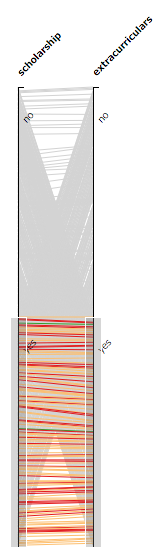
\includegraphics[width=0.2\textwidth]{scholarshipandextracurriculars}
\caption{ The subset of examples that participates in extracurriculars and has scholarship is highlighted. There are slightly more B examples, which are represented by the colored lines, than other grades. }
\label{featureselectiontask1}
\end{figure}

\begin{table}[]
\centering
\begin{tabular}{lc}
\hline
Answers & Frequency \\ \hline
A       & 5       \\
B       & 12         \\
A, B    & 3        \\ \hline
\end{tabular}
\caption{The frequency of the answers. Most participants were able to correctly identify B students as the most frequent target label.}
\label{InterpretFS1}
\end{table}

\subsubsection { Identify Features Separating Two Target Labels }

Second, participants were asked to identify features that distinguish or separate A from F students and those that distinguish B and C students.  To distinguish label u from label v, for each feature, we calculate the ratio of the more frequent label to less frequent label for each feature value. If the ratio is 4 or greater for each of feature value (meaning there is 4 times more of the frequent label than the less frequent label for each feature value), then we say that for the purpose of this task, the feature distinguishes label u from label v.

For A and F students, study time, extra classes, college, and scholarship were distinguishing. For B and C students, only scholarship, college, and study time were distinguishing. We calculated how many distinguishing features participants were able to identify.

Before group B participants started this task, they were first asked which features they thought could be causes or effects of student grades. We noticed that group B participants were likely to identify a distinguishing feature when the feature was previously identified by the participant as being a cause or effect of the target. Participants were relying on their intuitions about what features are important (causal features may be biased as important) to answer these questions. This behavior supports our design of incorporating prior knowledge into the feature selection process.

Participants did not identify all features that distinguish A from F and B from C students. The number of features identified by participants of each group is shown in table \ref{DistinguishingFeatures}. There may be many reasons why participants were not able to identify all distinguishing features. For example, some participants commented that the color associated with a label was visually stronger than that of another label. A subset of the participants utilized the filter for feature value functionality. Most participants utilized class label selection function to filter for the label(s) of interest; they observed the density of colored lines to determine whether a feature distinguishes the two labels/colors. Although there were eleven features and it was feasible to individually assess each feature, participants likely evaluated the entire graph to determine which features clearly separates the two colors. Moreover, for datasets with a larger number of features, we expected a user to be less likely to assess individual features and therefore the user is likely to not identify every distinguishing feature.

A participant commented that they had difficulties identifying patterns in the feature selection graph because the placement of the feature affects the visual. The placement of the feature may obscure the correlation between a feature value and another feature that is placed further away. The participant attempted to figure out what pairs and groups of features distinguish A from F labeled examples by rearranging feature axes; however, they stated they can not exhaust all possible rearrangement of axes. Other participants also commented that it was easier to identify the correlation between feature values when the feature axes were placed next to each other. The placement of the feature axes may be a contributing factor to why a feature was or was not identified as separating two target labels. Although visualization is a more efficient presentation of data, some information may be obscured. This is a ubiquitous challenge in data visualization. We have to sacrifice some clarity and certainty for the efficiency in visual data processing. We recognize that the uncertainty and ambiguity in the visual may increase with the increase in the number of examples and features in the dataset.

The average number of features distinguishing two class labels that the groups of participants identified is presented in table \ref{DistinguishingFeatures}. There is no significant difference between the number of features group A and group B participants are able to identify. However, group B participants behavior supports that causality may be a factor in identifying distinguishing features. Perhaps with a dataset with many more features, it would be more difficult for participants to rely solely on their intuitions about cause and effect relationships and would need help to obtain a complete picture of the causal relationship.

The average amount of time in minutes for participants to answer questions about patterns in the dataset is presented in table \ref{AvgTimeIdentifyPattern}. Participants were able to complete the task in an efficient manner by interpreting and interacting with the visualization. Identifying patterns or correlation between feature values might be more time consuming if the participants were presented with a table of the data or would require knowledge about data science which some of the participants did not have.

\begin{table}[]
\centering
\begin{tabular}{lc}
\hline
Participants & Avg Time (min) \\ \hline
CS (A)         &    10.7  $\pm$ 3.5        \\
Other (A)        &  14.7 $\pm$ 4.6           \\
\textbf{All (A)} & \textbf{12.3 $\pm$ 4.3}    \\ \hline
CS (B)         &    9.0 $\pm$ 5.1        \\
Other (B)        &  11.8  $\pm$ 2.3          \\
\textbf{All (B)} & \textbf{10.3 $\pm$ 3.9}   \\ \hline
\end{tabular}
\caption{The average amount of time for participants to complete the task of identifying patterns}
\label{AvgTimeIdentifyPattern}
\end{table}

\begin{table}[]
\centering
\begin{tabular}{lcc}
\hline
Participants & A and F (4) & B and C (3)\\ \hline
CS (A)       & 2.3 $\pm$ 0.5     & 1.3 $\pm$ 1.0        \\
Other (A)    & 1.8 $\pm$ 1.0      & 1.3  $\pm$ 0.8     \\
\textbf{All (A)} & \textbf{2.1 $\pm$ 0.7}        &  \textbf{1.8 $\pm$ 0.9}       \\ \hline
CS (B)       & 2.5 $\pm$ 0.8      &  1.8 $\pm$ 0.5       \\
Other (B)    & 1.8 $\pm$ 0.8     & 1.5 $\pm$ 0.6      \\
\textbf{All (B)} &   \textbf{2 $\pm$ 0.8} & \textbf{1.7 $\pm$ 0.5}        \\ \hline
\end{tabular}
\caption{The average number of features that were correctly identified as distinguishing A from F and B from C labels.}
\label{DistinguishingFeatures}
\end{table}

\subsection { Analyze Feature Set Metrics }
All the participants were able to determine how many Markov blanket features were covered in the feature selection by reading the Markov Blanket Consistency Chart. In addition, participants were able to determine whether importance features were in the feature selection. A participant explained that they used the Feature Importance Consistency Pie Chart to look at whether ``the green outer boxes corresponding to dark blue boxes", while others cited the rank loss score since higher loss means less consistency.

Some participants noted that feature analysis allowed them to refine their feature selection. A participant commented that when they ``ended up not being very consistent with the causal graph nor with the feature importance selection" which results in them changing their feature selection.

\subsubsection { Compare Feature Set Metrics }
Participants were able to describe the differences in feature analysis metrics between their current feature selection and trial 0, such as the MB score of trial 0 is greater than trial 1 and the rank loss of trial 0 is less than trial 0. However, 8 of the 15 participants did not explain the difference.

\subsubsection { Compare Classifier Performance }
Participants connected or explained a classifier's performance using feature analysis metrics. A participant, who demonstrated a clear understanding of the meaning of the feature metric, related feature metric to the performance of the classifier. They stated that trial 9 had only half of the Markov blanket features hence MB score of 0.5 and may be a reason why trial 9 's feature selection was not as great as trial 0 ’s.
Participants also used feature analysis metrics to help explain why a classifier may perform better than another classifier. For example, a participant explained that trial 1 performed worse than trial 0 because in trial 1 ``the selected features didn't cover all of the contributing factors to grades (hence the low MB coverage score) and weren't the most important". Moreover, a participant commented that trial 1 was ``not very consistent with the causal graph nor the feature importance selection" and attributed those characteristics to the low performance of the classifier.

Some participants commented that they utilized the feature analysis graphs and metrics influence a feature addition or removal.

\subsubsection { Participant Comprehension of Feature Metrics}
The participants demonstrated a good understanding of feature analysis metrics. From the comments on comparing classifiers, participants understand that a lower rank loss, higher MB score, and higher MI score may be the reason for a feature selection that creates a higher performing classifier than another selection. However, not all participants demonstrated that they understand how rank loss score and MB score connected to previously expressed prior knowledge.

Some participants did not understand the concept of Markov blanket coverage. For example, a participant mentioned, “sometimes removing Markov features from a feature selection did not remove the feature from being covered during the feature analysis”. These participants may have thought a feature in the Markov blanket Chart as covered if the feature was in the selected feature set. The concept of coverage was explained in the introductory material but may still be foreign to the participants. The concept can be better explained in the future.

\subsection{ Explore Feature Space}
In this section, we describe how participants in groups A and B explore the feature space and compare and contrast their behaviors.
\begin{table}[]
\centering
\begin{tabular}{lcc}
\hline
                 & CS  \\ \hline
avg \# of trials (A) &  7.3 $\pm$ 3.9        \\
total time (A)       &  13.3 $\pm$ 3.4       \\
\textbf{time per trial (A)}   &  \textbf{2.5 $\pm$ 1.5}         \\ \hline
avg \# of trials (B) &  11  $\pm$ 5.7      \\
total time (B)       &  13.8  $\pm$ 9.0      \\
\texbf{time per trial (B)} &  \textbf{1.3 $\pm$ 0.7}          \\ \hline
\end{tabular}
\caption{The average number of trials completed by group A and B participants and the time spend on the task. }
\label{versionAvsversionB}
\end{table}
\subsubsection { Group A Observations }
Group A participants start with the feature set of target Markov Blanket features in the feature selection. Participants then make minor changes to the Markov blanket feature set. They make elementary changes to the Markov blanket feature set such as adding or removing a feature from the default feature set. Feature additions are more common than feature removals. Initially, participants do not deviate far from the Markov blanket feature set with some exceptions.

Some participants commented that they analyzed the feature analysis before creating the classifier. After a feature was added or removed, they reviewed the feature metrics which influenced whether the change was reversed or not. Group A participants demonstrated that they understand the feature metrics and know how to compare feature metrics of different feature selections. A participant noted that when they saw that a feature selection had a lower MB and MI score than trial 0, the participants changed the feature selection before creating a classifier.
Participants compared their feature selection to trial 0 and aimed to get a better MI score and/or lower rank loss score. Group A also performed fewer trials than group B. Group A was most likely ruling out certain feature sets because of feature metric scores. They were more likely to focus on a subspace of feature sets because of the metrics.

\subsubsection { Group B Observations }
Group B participants were shown an empty set because prior information was not communicated to the system. Before they made feature selection, they were asked which features they thought could be causes or effects of student grades.

Participants relied on their intuition when selecting features and often selected features that they think are causal. When causal discovery is not integrated, participants have to rely on their instincts to figure out which features influence the target. However, participants identified different causal features and initial feature selections varied greatly. By incorporating causality, we can help the user identify causal features that may be predictive.

Moreover, by incorporating causality, participants could identify causal features that they may not have thought about. For example, while participants were able to identify direct causes and effects, they were less equipped to identify indirect influences. GES could provide participants with a complete picture of causal relationships; the visual could help people identify indirect influences to the target that may help build a high performing classifier.

On the other hand, some participants did not start with features that they identify as causal. They started by creating a classifier with a small set of features and added and removed features based on the accuracy of the resulting classifier.

\subsubsection { Group A vs Group B }
Group A participants on average spent more time between trials. Group A participants may be putting in more thought or reasoning about their selected feature set. They may be spending more time between trials because they could evaluate metrics describing the consistency of the feature set. Many participants commented that they review the feature analysis metrics when making feature selections. Some group A participants completed only a few trials in a long stretch of time.

On the other hand, group B participants completed many trials in a similar period of time. Group B participants were more likely to use guesswork when selecting features. Moreover, group B participants did not start with a default feature selection and did not have additional metrics to guide their selection. They rely on their intuition and trial and error. Initial feature sets were usually features they think are causal. Then they remove and add features based on whether the accuracy of the classifier improves.

Trial and error is also a common technique in group A and group B. Participants added or removed features from the selected feature set. Some group A participants did not proceed to create a classifier with that feature set if the metrics are low. For example, most group A participants have 4 or more features in all their trials because the size of their default feature selection is 4 or more and a feature set with less than 4 features would have a low Markov blanket feature score consistency.

On the other hand, group B participants have to verify their intuition and whether they selected predictive features by creating a classifier. As a result, group B participants create more classifiers and also start with a smaller set of selected features.

Another trial and error technique observed in both groups is to remove and add features to the highest performing classifier. 6 (40\%) group A participants and 5 (50\%) group B participants In both groups, the accuracy does not go up continuously. The system stores the iterations of the feature sets and the classifiers and provides graphs to display the progress. Participants were able to compare performances of different iteration. They can then choose to select a previous iteration that performed better and make elementary changes to that feature set. The system is designed for the iterative process of classification and incorporates visuals for comparing performances of different iterations and stores information about previous information. These observations support that the iterative design helps the participants search for high performing classifiers by allowing them to search a subspace of predictive feature sets and comparing feature sets.

We argued that incorporating human’s soft knowledge would be beneficial to the feature selection process. However, we need to be able to leverage their prior knowledge, visual, and analytical capabilities. In version B, although participants were able to recall features they thought may influence student grades, they had to rely mainly on trial and error to test their knowledge. On the other hand, in version A, participants were able to communicate to the system through visuals which features they thought were important. The system and the participants were able to collaboratively build a causal graph; the causal algorithm provided the participant with a possible picture of causal relationships based on suggestions from the participant about which features were important and the participants then correct the graph to more closely reflect their prior knowledge. As a result, group A participants got a more accurate and complete image of the causal relationship. Group A participants also started ahead of group B participants because they started with a set of causal features while group B started with the empty set. Group A had to verify whether the causal features were predictive, while group B had to verify that the feature they thought was important was actually predictive.

Moreover, results from both groups demonstrated the efficiency and usability of the interface and interactions. Participants did not have trouble dragging the feature axes to select features. All participants were able to attempt several trials in less than 30 minutes before deciding on the feature set to predict the target. The amount of time the participants in group A and B spent exploring the feature space is presented in table \ref{versionAvsversionB}.

\subsection { Feature Selection Iterations }
\begin{figure}
    \centering
    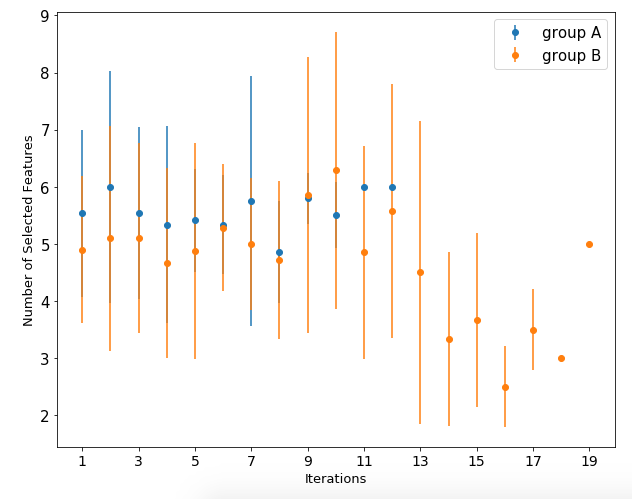
\includegraphics[width=.75\textwidth]{numberofselected}
    \caption{\textbf{Number of Features Selected}. The average number of features selected in each iteration by group A and group B. Group A feature set sizes tend to be bigger than that of Group B in the first 5 trials.  }
    \label{fig:numberofselected}
\end{figure}

\begin{figure}
    \centering
    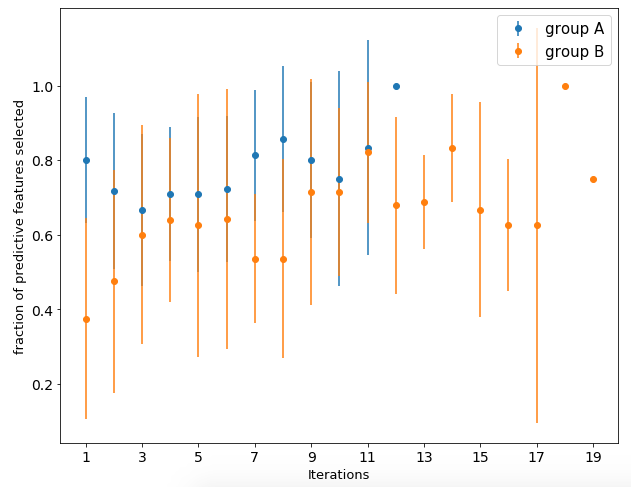
\includegraphics[width=.75\textwidth]{predictivefeaturesselected}
    \caption{\textbf{Fraction of Predictive Features Selected }. The average fraction of the predictive features that was selected in each iteration by group A and group B. On average, group A had more predictive feature in its feature set than group B. }
    \label{fig:predictivefeaturesselected}
\end{figure}

\begin{figure}
    \centering
    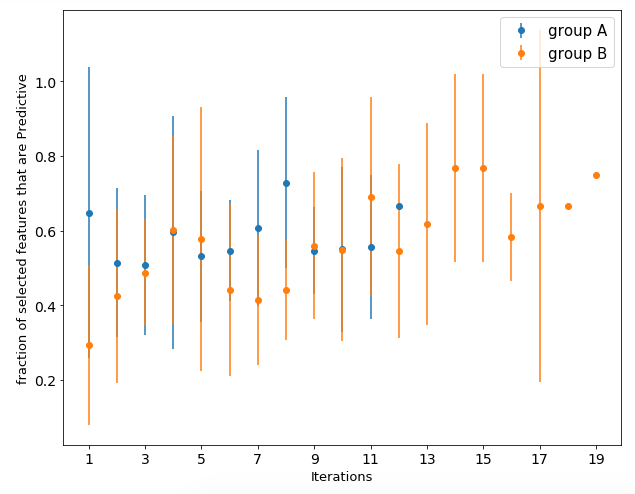
\includegraphics[width=.75\textwidth]{selectedfeaturethatarepredictive}
    \caption{\textbf{Fraction of Selected Features that is Predictive }. The average fraction of the selected feature set that is predictive in each iteration for group A and group B. On average, a bigger fraction of group A's selected feature set is predictive. }
    \label{fig:selectedfeaturethatarepredictive}
\end{figure}

We compare the feature selection behavior of group A and group B. 

The average number of features selected per iteration for group A and group B is plotted in figure \ref{fig:numberofselected}. Group B tend to have smaller feature sets than group A in the first seven trials. This may be because group A started with the set of MB features of the target which can range from 4 to 7 features depending on the causal graph built by the participant. Moreover, the error bars are larger in the first few iterations for group A because some participants removed features while other added features to the set of MB feature. 

The fraction of predictive features selected per iteration by group A and group B is plotted in figure \ref{fig:predictivefeaturesselected}. On average, group A selected more predictive features than group B. Moreover, the error bars for group B are larger which indicates that group B's feature selection behavior varies greater than group A's. 

The fraction of selected features per iteration that are predicted for group A and group B is plotted in figure \ref{fig:selectedfeaturethatarepredictive}. On average, a larger fraction of the selected features is predictive for group A. Moreover, group B starts with a small fraction of the selected features as predictive because group B had to guess and check for predictive features. On the other hand, some of the MB features are predictive so group A starts with a higher fraction of the selected features as predictive. 

\subsection { Effectiveness of Feature Selection }
The irrelevant features in the dataset are motherhasjob, fatherhasjob, age. The causal graph should reveal that these features are irrelevant. Age does not have an edge to or from any of the features which indicates that it is not related to any of the features. Motherhasjob and fatherhasjob are features that do not have a directed path to or from the target variable.

Building the causal graph and expressing feature importance can help reveal predictive features to the participants. For example, study time and college are predictive features and are indicated as more important than the others during the feature importance step.

Furthermore, in the original graph built by GES, the target's Markov blanket contains many predictive features. For example, scholarship, study time, family support, and extra classes are likely to be in the target Markov blanket and are predictive features.

The original graph output by GES could be changed by ranking other features as most important during the expressing feature importance step. From the few participants who ranked other features as most important, the feature they indicated as most important was already in the Markov blanket of the target even if they did not make that indication. Moreover, a participant could change the relationships between the target and a feature in the causal graph which could result in a change in the target's Markov blanket. However, participants did not remove edges to or from the target and more likely to reverse edges which likely adds features to the target's Markov blanket. Therefore, the predictive features were likely to be in the target's Markov blanket when the participant proceeds to the feature selection step.

The feature selection step can also help uncover predictive features. For example, scholarship is predictive and separates both A from F students and B from C students. In addition, study time separates B from C students and is predictive. However, it is noted that not all the participants were able to identify scholarship and/or study time as a distinguishing feature in the previous step; on average, group A and B participants identified about 2 of the 4 features distinguishing A from F and 2 of the 3 features distinguishing B from C.

Relevant feature sets and their testing accuracy are reported in table \ref{relevantFS}.

\begin{table}[]
\centering
\begin{tabular}{ll}
\hline
Feature Sets                                               & Accuracy \\ \hline
extra classes, family support, scholarship, study time (4) & 0.886    \\
extra classes, college, family support, study time (4)     & 0.876    \\ \hline

\end{tabular}
\caption{Predictive feature sets and the accuracy of their classifiers}
\label{relevantFS}
\end{table}

\subsection { Group A Best Feature Selection }

\subsubsection { Likely to include important features }
All but two participants or about 86\%, included study time in their final feature selection as shown in table \ref{RelevantFSBasedOnImportance}. Study time is expressed as the most important feature during the expressing feature importance step. Study time is indicated as an important feature in the Feature Importance Consistency Chart and including it would lower the rank loss score. The most likely reason why study time is in the feature selection is that it was in the Markov blanket of student grade and in the default feature selection. Therefore, the important features indicated by the participant is taken into account when creating the causal graph and making the default feature selection. This helps the participant and the system filter for predictive features.

On the other hand, college was expressed as the second most important feature by all participants. Only 6 participants or about 40\% included college in the final feature selection. It is not in the target's Markov blanket for most of the participants and therefore, not in the default feature selection. This makes it less likely to be in the final feature set.

Most of group B participants also included study time. Most likely because many participants (80\%) thought study time influences student grades. Moreover, many participants (60\%) are able to see that study time separates A from F students or B from C students. Therefore, the feature selection graph can also help participants visually identify predictive features.

\subsubsection { Likely to exclude irrelevant features }
All but 1 participants or about 93\% excluded motherhasjob and fatherhasjob in their final feature set with the exception of a participant who included all the features in their final feature selection, as shown in table \ref{IrrelevantFeatures}. In addition, all participants but two excluded age. Most participants did not include all three features in their trials. This is most likely because they were not apart of the target's Markov blanket and did not have a direct path to or from student grade in the causal graph. Causality is able to help participants filter out irrelevant features.

\subsubsection { Likely to include Markov blanket features }
Group A participants are likely to include Markov blanket features in the final feature set. The final feature set contains may Markov blanket features. On average 75\% of the final feature selection consists of the target's Markov blanket features. At least three of the features in the feature selection are Markov blanket features of the target.

All but three participants include scholarship, which is a predictive feature, in their final feature selection. This is more likely because scholarship is in the default feature selection. Participants also observed that removing scholarship, without replacing it with college, would decrease the performance of the classifier and the Markov blanket score. Of the participants that did not include scholarship, all included college except from one, which shows that they are able to cover scholarship by including college.

Expressing prior information about feature importance and causal relationships help find predictive features.

\begin{table}[]
\centering
\begin{tabular}{lccc}
\hline
Participants & \multicolumn{1}{l}{age} & \multicolumn{1}{l}{mother has job} & \multicolumn{1}{l}{father has job} \\ \hline
group A      & 1 (6.6\%)                &  1 (6.6\%)     &  1 (6.6\%)                                  \\
group B      & 1 (10\%)                 &  1 (10\%)   & 0 (0\%) \\\hline
\end{tabular}
\caption{The number of participants in each group that included the irrelevant features.}
\label{IrrelevantFeatures}
\end{table}

\begin{table}[]
\centering
\begin{tabular}{lccc}
\hline
Participants & \multicolumn{1}{l}{study time} & \multicolumn{1}{l}{college} & job \\ \hline
group A      & 13 (87\%)                      &  9  (60\%) & 13 (87\%)               \\
group B      & 8 (80\%)                       &  6  (60\%) & 3  (30\%)          \\ \hline
\end{tabular}
\caption{The number of participants that included the important and causal feature in their feature selection.}
\label{RelevantFSBasedOnImportance}
\end{table}

\begin{table}[]
\centering
\begin{tabular}{lccc}
\hline
Participants & \multicolumn{1}{l}{scholarship} & \multicolumn{1}{l}{extra classes} & \multicolumn{1}{l}{family support} \\ \hline
group A      & 13 (86\%)   & 6 (40\%)  & 9 (60\%)  \\
group B      & 8 (80\%)     & 6 (60\%)  & 6 (60\%)  \\ \hline
\end{tabular}
\caption{The number of participants that included the feature in their best feature selection.}
\label{RevelantFSBasedOnCausal}
\end{table}

\subsection{Evaluating Feature Sets}
When the participant was asked whether their final selection of features was intuitive, the participant used cause and effect relationships to explain why the features may be predictive of the target. For example, they stated that college and scholarship are predictive because ``college, scholarship are all affected by grade." This shows that users rely on causal relationships they think may exist in the dataset when selecting for features. Furthermore, a participant who has taken a course on machine learning knew to remove redundant features. They stated that ``mother job and father job will influence the family income, and the family income will have an effect on family support. They both have similar influence for grade, so we only necessary pick family support." They understood that the improvements to the classifier will be minimal when adding the features, motherhasjob, and fatherhasjob because their influence on the target is captured in family support.

\subsection { Performance of Classifiers }
The performances of the classifiers created by group A and B are similar. This is because the size of the dataset allows for group B participants to filter for predictive features by trial and error. There are only 11 features and the time to create a classifier is nearly immediate. As a result, group B participants are able to go through many trials and pick out predictive features through trial and error and intuition.

However, we notice differences in the feature selection behaviors of both groups. Group A participants are more likely to spend more time between trials and review the feature analysis metrics before creating a classifier - group A participants averaged 2.5 minutes per trial and group B participants averaged 1.3 minutes per trial. As a result, they create fewer trials and are able to identify a high performing feature set in less trial than group B participants - group A averaged 7.3 trials while group B averaged 11.0 trials. Feature analysis metrics may have helped them identify good sets of features.

Moreover, for a larger dataset with more features, the time to create a classifier will increase. Trial and error will not be a reliable strategy, and the user can not rely on their intuition alone to initially find a good set of features. On the other hand, the user's prior knowledge and complete causal graph help the system and the user focus on a subspace of feature sets and be less likely to go down a rabbit hole. The user can utilize feature analysis metrics to access a feature set before creating a classifier which will only get more time consuming with the complexity of the dataset.

\begin{table}[]
\centering
\begin{tabular}{lcc}
\hline
Participants & \multicolumn{1}{l}{Size of Feature Set} & \multicolumn{1}{l}{Testing Accuracy} \\ \hline
group A      &  5.8 $\pm$ 1.9    &  0.811 $\pm$ 0.008        \\
group B      &  6.0 $\pm$ 2.5  &    0.818 $\pm$ 0.004        \\\hline
\end{tabular}
\caption{Average size of feature size and average accuracy of classifier created from best feature selection}
\label{AccuracyComparison}
\end{table}

\begin{table}[]
\centering
\begin{tabular}{ll}
\hline
Feature Selection Method & Features                                                 \\ \hline
Mutual Information       & college, scholarship, studytime, job, extraclasses       \\
Markov Blanket           & scholarship, familysupport, extraclasses, studytime, job \\ \hline
\end{tabular}
\caption{The features selected by other feature selection methods.}
\label{otherFSmethods}
\end{table}

\begin{table}[]
\centering
\begin{tabular}{lll}
\hline
Feature Selection Method & Feature Set Size & Accuracy \\ \hline
Mutual Information       & 5                & 0.814    \\
Markov Blanket           & 5                & 0.812    \\
group A      &  5.8 $\pm$ 1.9    &  0.811 $\pm$ 0.008        \\
group B      &  6.0 $\pm$ 2.5  &    0.818 $\pm$ 0.004        \\\hline
\end{tabular}
\caption{The feature size and performance of feature sets selected by different feature selection methods.}
\label{otherFSperformance}
\end{table}

\subsubsection { Compare to Other Feature Selection Methods }
We compare the average performance of the feature sets selected by group A and B against the performance of feature sets selected by other non-interactive algorithms, such as mutual information based feature selection and causal feature selection. The features that share the highest amount of information with the target variable are college, scholarship, studytime, job, extraclasses, as reported in table \ref{otherFSmethods}. The accuracy of the classifier using those features is 0.814. In addition, in one causal network generated by GES, the MB of student grade consists of scholarship, familysupport, extraclasses, studytime, job, as shown in figure \ref{fig:Task2} and table \ref{otherFSmethods}; the classifier's accuracy is 0.812. 

Group A and group B did no better and no worse than mutual information based feature selection and causal feature selection. As shown in table \ref{otherFSmethods}, all feature selection methods resulted in classifiers with similar performance. There may be no significant difference in the results because the dataset used the evaluation study may be too trivial and small. The collaborative features selection method did no worse than the other two methods we compared against which shows that our method may help people select predictive features as well as make sense of the predictive feature set. 
